\section{Mathematical Models}
\label{ch:mathmodel}

As per the base and periodic models shown in \cite{grigor20}.

\subsection{Base model}

\subsubsection{Definitions and Theory}

\subsubsection{How to select the best model}

\begin{figure}[H]
\minipage{0.33\textwidth}
  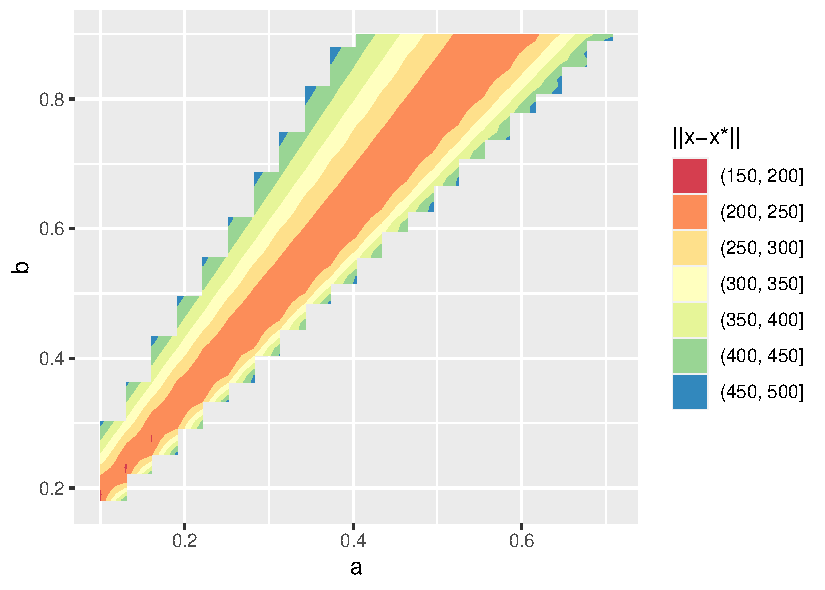
\includegraphics[width=\linewidth]{Ireland-combnorm.pdf} \label{fig:ireland-combnorm}
\endminipage\hfill
\minipage{0.33\textwidth}
  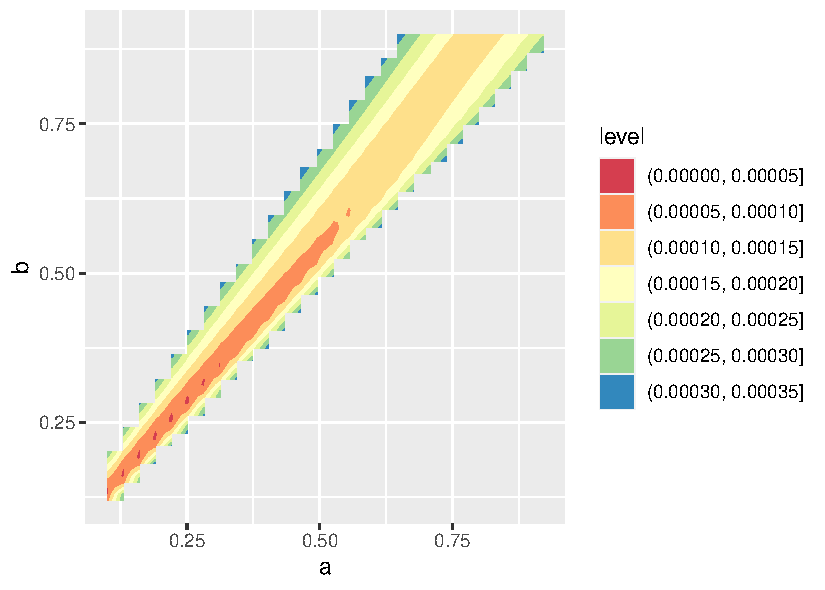
\includegraphics[width=\linewidth]{Italy-combnorm.pdf} \label{fig:italy-combnorm}
\endminipage\hfill
\minipage{0.33\textwidth}
  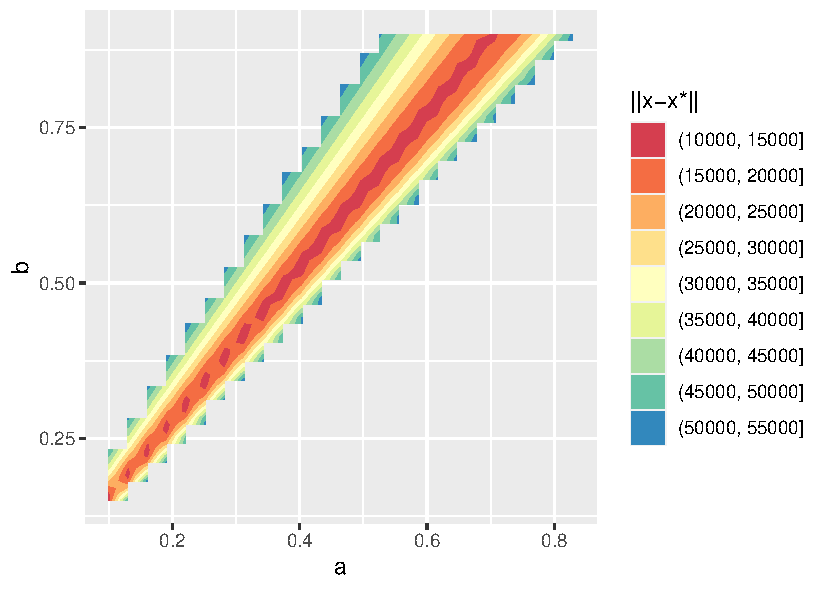
\includegraphics[width=\linewidth]{United States-combnorm.pdf} \label{fig:usa-combnorm}
\endminipage\hfill
\caption{Contour plots of $||x-x^*||$, Ireland, Italy and United States}
\end{figure}

\subsubsection{Forecasting}

\subsubsection{Implementation in R}

\subsubsection{Plots}

\begin{figure}[H]
\minipage{0.48\textwidth}
  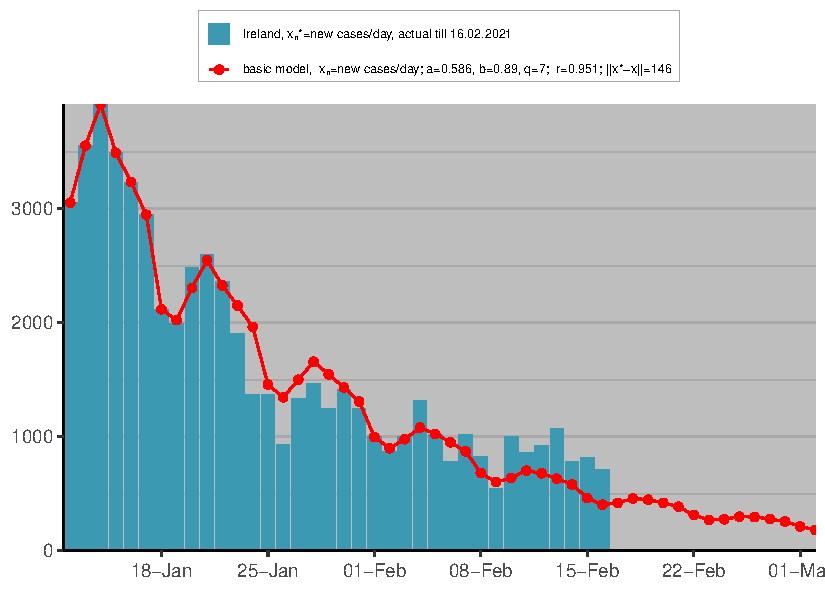
\includegraphics[width=\linewidth]{Ireland-basexn.pdf} \label{fig:ireland-basexn}
\endminipage\hfill
\minipage{0.48\textwidth}
  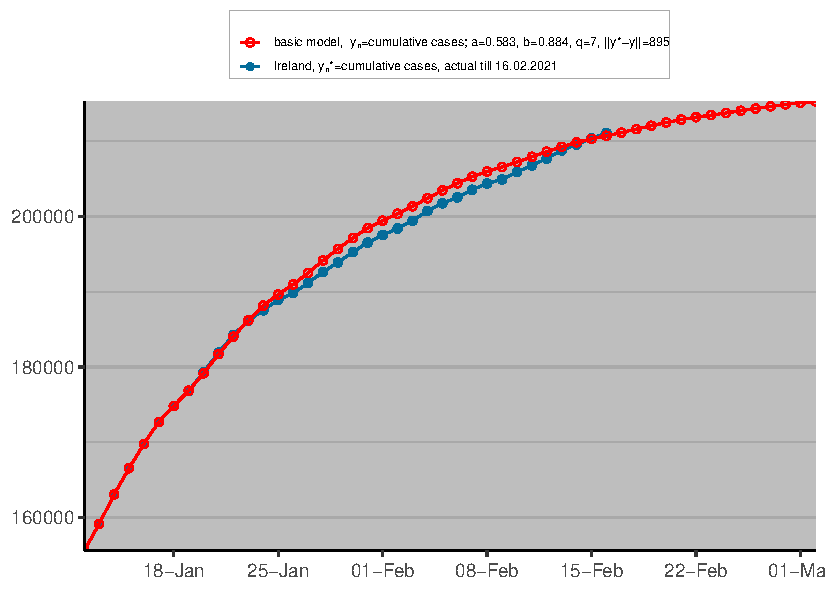
\includegraphics[width=\linewidth]{Ireland-baseyn.pdf} \label{fig:ireland-baseyn}
\endminipage
\caption{Basic model, Ireland}
\end{figure}

\begin{figure}[H]
\minipage{0.48\textwidth}
  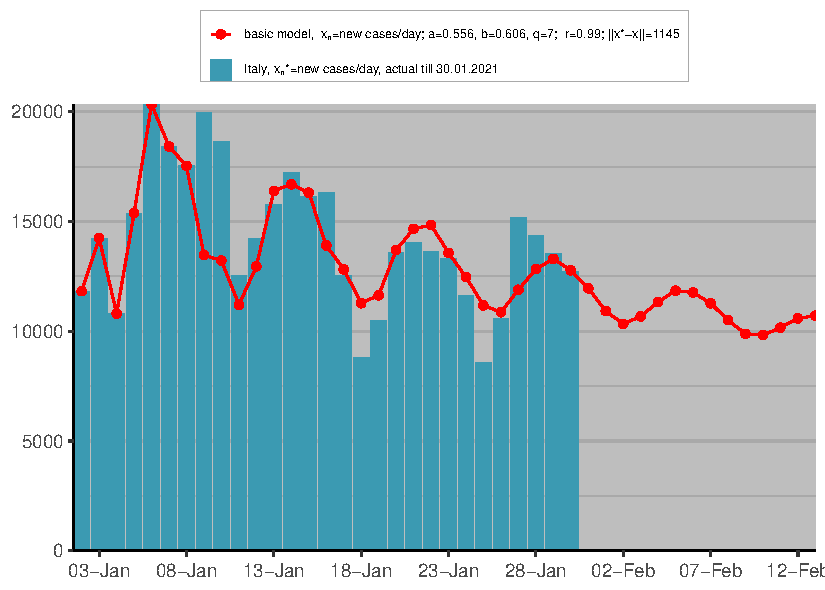
\includegraphics[width=\linewidth]{Italy-basexn.pdf} \label{fig:italy-basexn}
\endminipage\hfill
\minipage{0.48\textwidth}
  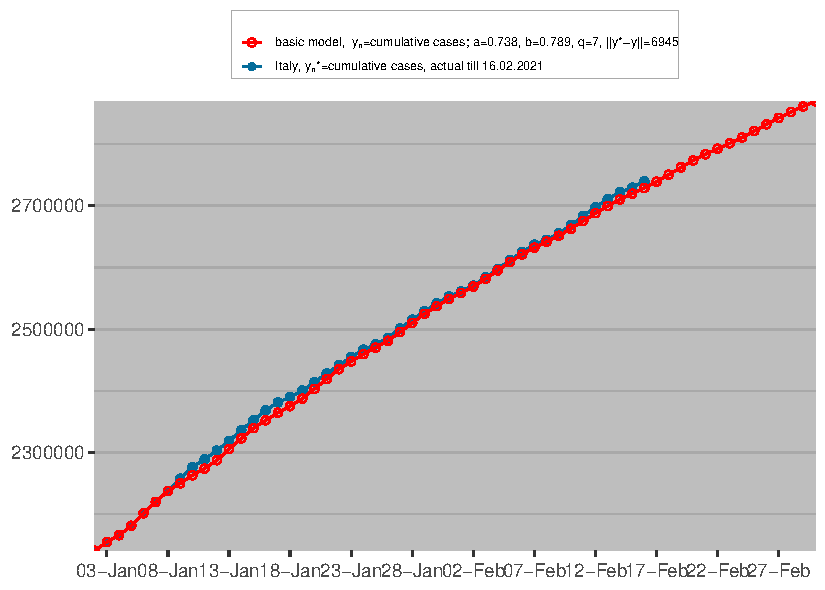
\includegraphics[width=\linewidth]{Italy-baseyn.pdf} \label{fig:italy-baseyn}
\endminipage
\caption{Basic model, Italy}
\end{figure}

\begin{figure}[H]
\minipage{0.48\textwidth}
  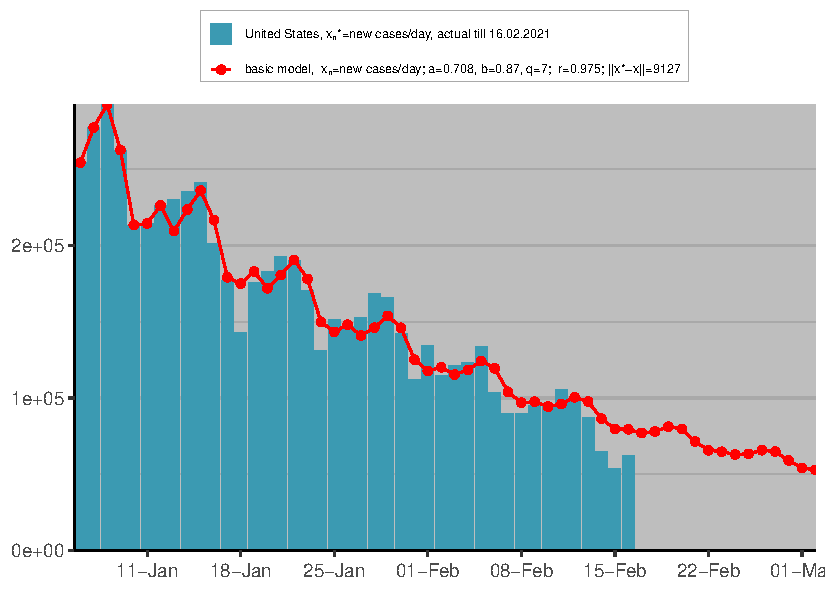
\includegraphics[width=\linewidth]{United States-basexn.pdf} \label{fig:usa-basexn}
\endminipage\hfill
\minipage{0.48\textwidth}
  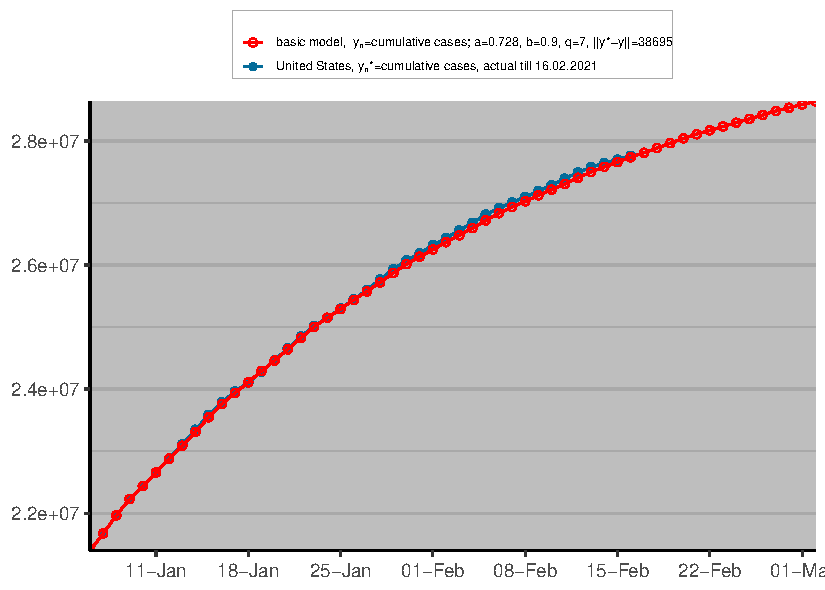
\includegraphics[width=\linewidth]{United States-baseyn.pdf} \label{fig:usa-baseyn}
\endminipage
\caption{Basic model, United States}
\end{figure}

\subsection{Limiting curve}

\begin{figure}[H]
\minipage{0.98\textwidth}
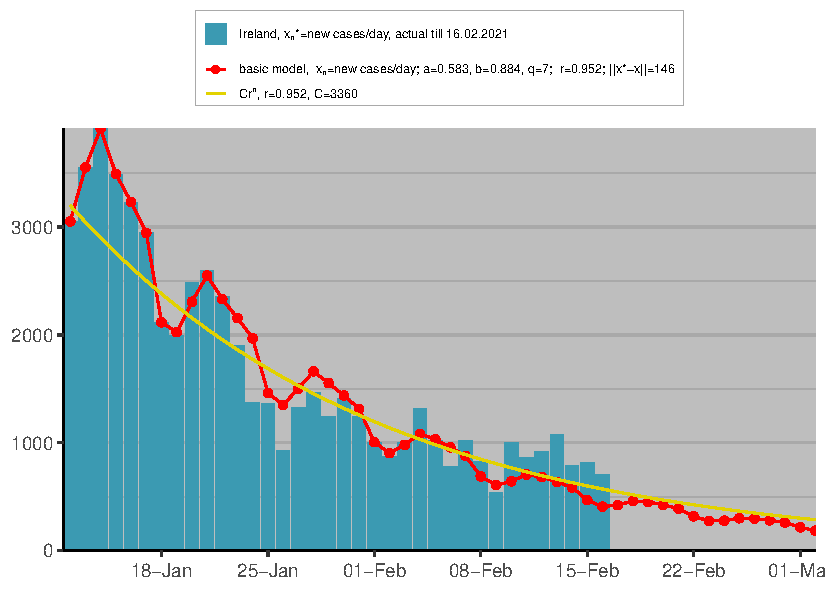
\includegraphics[width=0.9\textwidth]{Ireland-Crn.pdf}
\endminipage 
\caption{Comparison of $x^*_n,\ x_n$ and the limiting curve $Cr^n$, Ireland}
\end{figure}

\begin{figure}[H]
\minipage{0.98\textwidth}
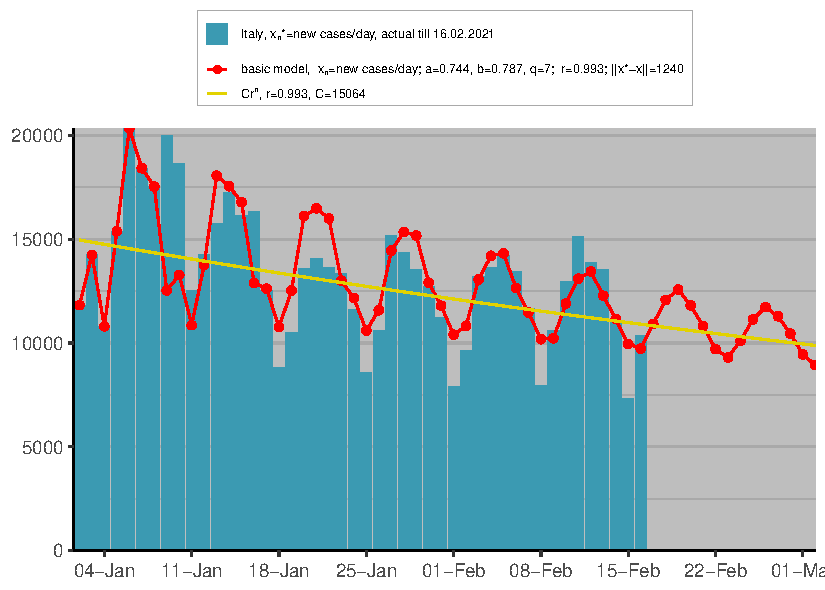
\includegraphics[width=0.9\textwidth]{Italy-Crn.pdf}
\endminipage 
\caption{Comparison of $x^*_n,\ x_n$ and the limiting curve $Cr^n$, Italy}
\end{figure}

\begin{figure}[H]
\minipage{0.98\textwidth}
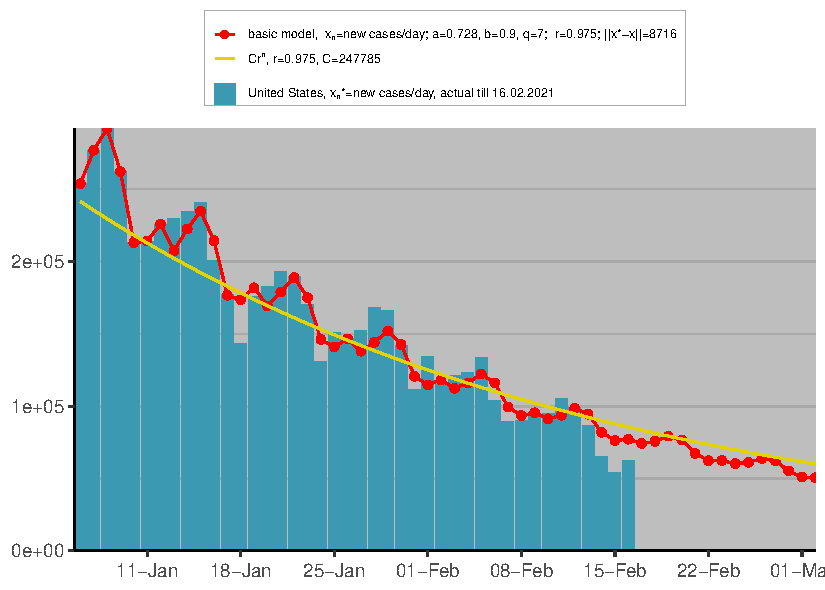
\includegraphics[width=0.9\textwidth]{United States-Crn.pdf}
\endminipage 
\caption{Comparison of $x^*_n,\ x_n$ and the limiting curve $Cr^n$, United States}
\end{figure}

The limiting curve can of course so exponential growth 

\begin{figure}[H]
\minipage{0.98\textwidth}
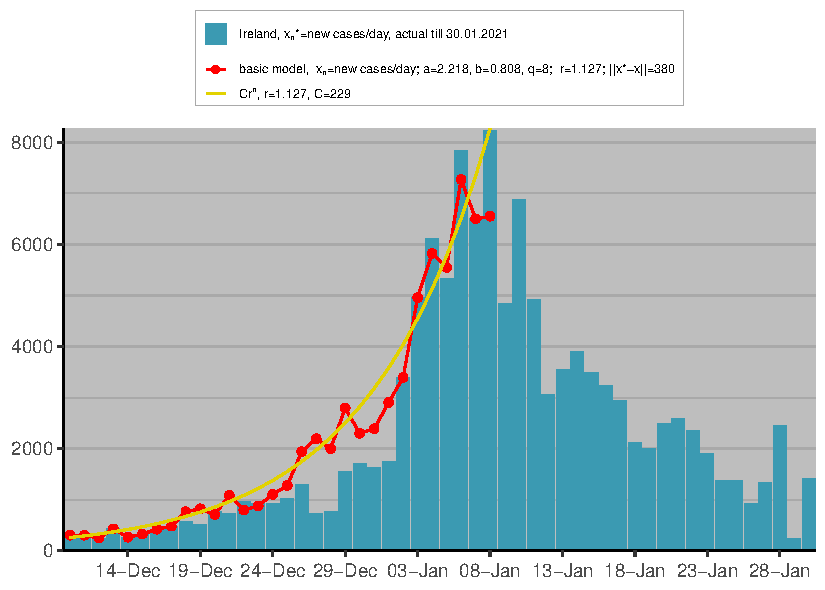
\includegraphics[width=0.9\textwidth]{Ireland-expgrowth.pdf}
\endminipage 
\caption{Limiting Curve Growing Exponentially, Ireland}
\end{figure}

\subsection{Moving average}

Define the $2k+1$-day moving average of actual data $x_n^*$ by $x^*(k)$

$\begin{aligned}
x^*_n(1) &=\frac{x^*_{n-1} + x^*_n + x^*_{n+1}}{3},\quad 1\leq n < N \\
x^*_0(1) &=\frac{x^*_0 + x^*_1}{2}\\
x^*_N(1) &=\frac{x^*_{N-1} + x^*_N}{2}
\end{aligned}$

And then $$x_n^*(3):= x^*_n(x^*_n(1))$$ is the 7-day moving average of cases.

Good baseline for model performance 

(want $\norm{x-x^*}\approx\norm{x^*(3)-x^*}$ or better)

\begin{figure}[H]
\minipage{0.98\textwidth}
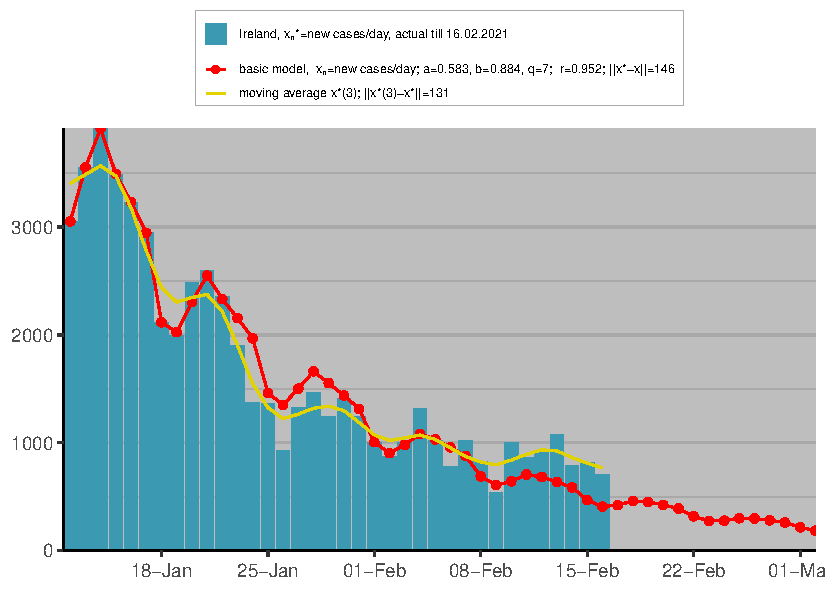
\includegraphics[width=0.9\textwidth]{Ireland-mavgx3.pdf}
\endminipage 
\caption{Moving average $x^*_n (3)$, Ireland}
\end{figure}

\begin{figure}[H]
\minipage{0.98\textwidth}
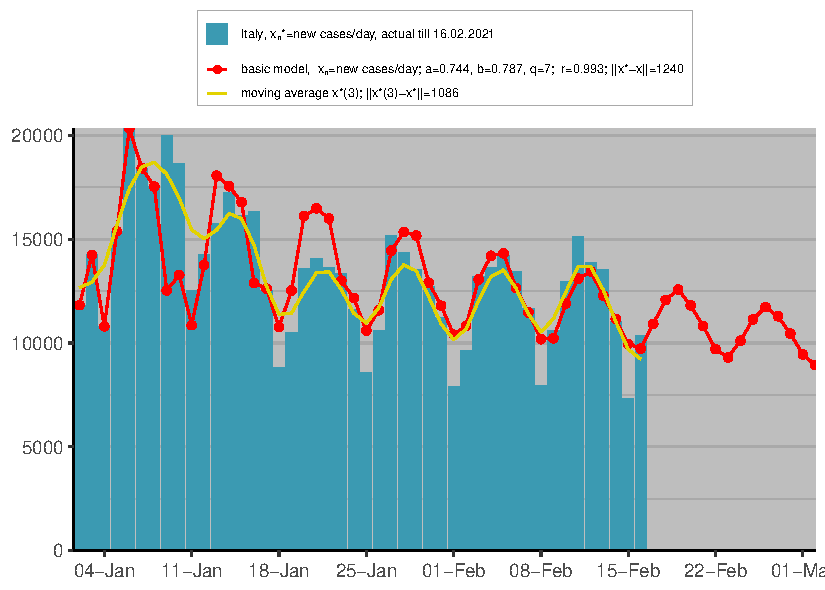
\includegraphics[width=0.9\textwidth]{Italy-mavgx3.pdf}
\endminipage 
\caption{Moving average $x^*_n (3)$, Italy}
\end{figure}

\begin{figure}[H]
\minipage{0.98\textwidth}
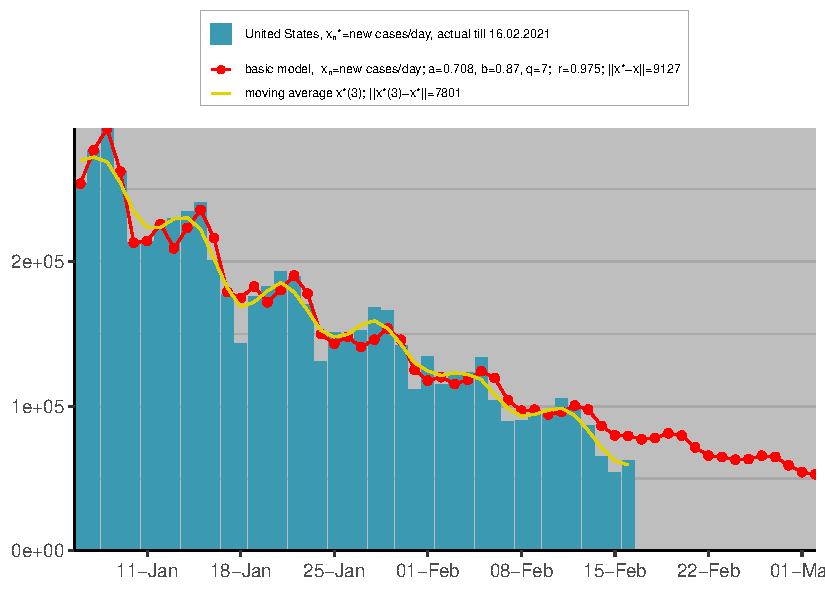
\includegraphics[width=0.9\textwidth]{United States-mavgx3.pdf}
\endminipage 
\caption{Moving average $x^*_n (3)$, United States}
\end{figure}

\subsection{Periodic model}

Instead of constant parameters $a,b$, we vary them slightly over time:

$a_n := a\rbr{1+c_1\rbr{\sin\rbr{\frac{2\pi}{p_1}\rbr{n-n_1}}}}$

$b_n := b\rbr{1+c_2\rbr{\sin\rbr{\frac{2\pi}{p_2}\rbr{n-n_2}}}}$

For new parameters $c_i,p_i,n_i, \ i=1,2$ where

$c_i  \in [0.04, 0.2] \quad \text{small}$

$n_i  \in 1,2,\dots,q$

$p_i  \in 1,2,\dots,q$

\begin{figure}[H]
\minipage{0.33\textwidth}
  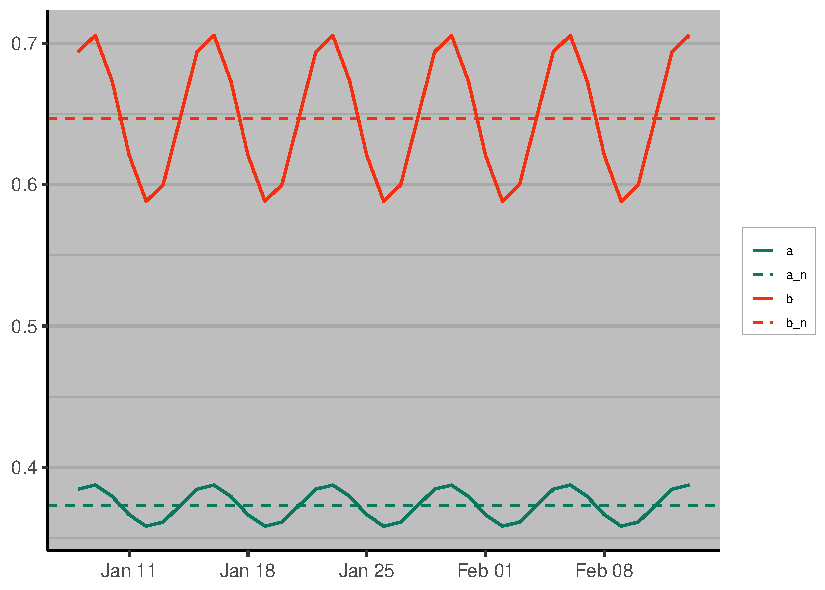
\includegraphics[width=\linewidth]{Ireland-perparam.pdf} \label{fig:ireland-perparam}
\endminipage\hfill
\minipage{0.33\textwidth}
  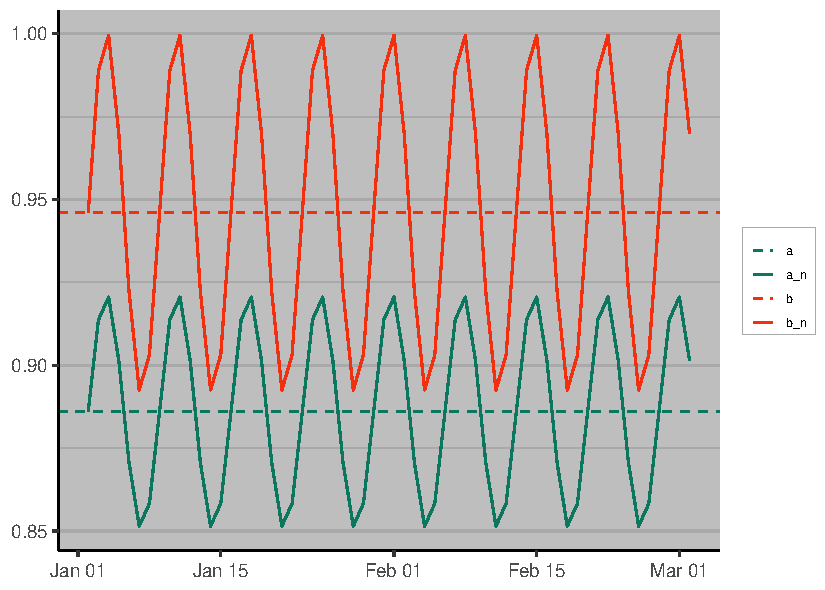
\includegraphics[width=\linewidth]{Italy-perparam.pdf} \label{fig:italy-perparam}
\endminipage\hfill
\minipage{0.33\textwidth}
  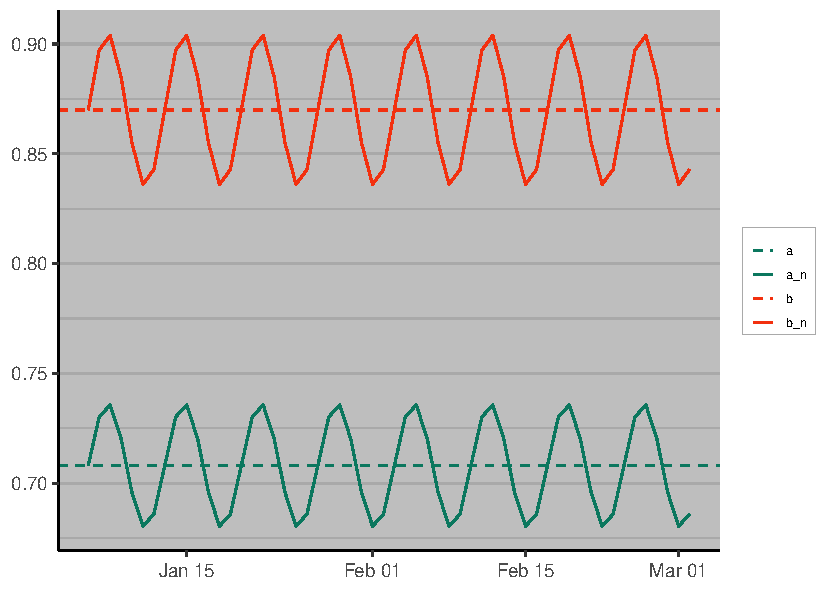
\includegraphics[width=\linewidth]{United States-perparam.pdf} \label{fig:usa-perparam}
\endminipage\hfill
\caption{Oscillating $a$ and $b$ parameters, Ireland, Italy and United States}
\end{figure}

\subsubsection{Definitions and Theory}

\subsubsection{How to select the best model}

\subsubsection{Forecasting}

\subsubsection{Implementation in R}

\begin{lstlisting}[frame=single, caption = {Algorithm for Periodic Model}]
modxper <- function(par, q, x, len = 0){
  #a,b,c1,c2,p1,p2,n1,n2
  an   <- par[1]*(1+par[3]*sin(2*pi*(1:(length(x)+len) - par[7])/par[5]))
  bn   <- par[2]*(1+par[4]*sin(2*pi*(1:(length(x)+len) - par[8])/par[6]))
  modx <- x[1:q]
  for(i in (q+1):(length(x)+len)){
    modx[i] <- (bn[i]*(1-bn[i-1]))*modx[i-1]/bn[i-1] +
      (an[i-q]*bn[i])*modx[i-q]/bn[i-q]
  }
  return(modx)
}

normper <- function(par, q, x) return(modnorm(x,modxper(par,q,x)))

#parameters of the form (ci,pi,ni)
  ##an = a(1 + c1 sin(2pi/p1 (n - n1)))
  ##bn = b(1 + c2 sin(2pi/p2 (n - n2)))
  aseqper <- a*seq(from = 0.8, to = 1.2, length.out = 5)
  bseqper <- b*seq(from = 0.8, to = 1.2, length.out = 5)
  c_1seq  <- c_2seq <- seq(0.04, 0.2, length.out = 10)
  n_1seq  <- n_2seq <- c(1,7)
  p_1seq  <- p_2seq <- 6:7
  normdatp <- expand.grid(a  = aseqper, b  = bseqper,
                          c1 = c_1seq,  c2 = c_2seq,
                          p1 = p_1seq,  p2 = p_2seq,
                          n1 = n_1seq,  n2 = n_2seq)
  
  pernorm <- apply(normdatp, 1, function(x) normper(x, q = q, countrydat$xn))
  normdatp$pernorm <- pernorm
  
  peroptim     <- normdatp[which.min(pernorm),1:8]
  optpernorm <- normdatp[which.min(pernorm),9]
  
  modeldat$periodic  <- modxper(as.numeric(peroptim),countrydat$xn, q = q, forecastlen)
  modeldat$periodicy <- xntoyn(modeldat$periodic) + prevcases
  
  optpernormy <- modnorm(countrydat$yn, modeldat$periodicy[1:nrow(countrydat)])
  
  peroptim <- round(as.numeric(peroptim),3)
   
  #a,b,c1,c2,p1,p2,n1,n2
  labs$periodic <- list(bquote("periodic model,"~x[n]*"=new cases/day;"
                              ~a*"="*.(peroptim[1])*","~ b*"="*.(peroptim[2])*","
                              ~q*"="*.(q)*";"~"||x*-x||="*.(optpernorm)*";"
                              ~c[1]*"="*.(peroptim[3])*","~p[1]*"="*.(peroptim[5])*","
                              ~n[1]*"="*.(peroptim[7])*","~c[2]*"="*.(peroptim[4])*","
                              ~p[2]*"="*.(peroptim[6])*","~n[2]*"="*.(peroptim[8])))
  
  labs$periodicy <- list(bquote("periodic model,"~y[n]*"=new cases/day;"
                               ~a*"="*.(peroptim[1])*","~ b*"="*.(peroptim[2])*","
                               ~q*"="*.(q)*";"~"||x*-x||="*.(optpernormy)*";"
                               ~c[1]*"="*.(peroptim[3])*","~p[1]*"="*.(peroptim[5])*","
                               ~n[1]*"="*.(peroptim[7])*","~c[2]*"="*.(peroptim[4])*","
                               ~p[2]*"="*.(peroptim[6])*","~n[2]*"="*.(peroptim[8])))
  
  plots[["periodic"]] <- plot_periodic(countrydat, modeldat, cols, labs)
  
  plots[["periodicy"]] <- plot_periodicy(countrydat, modeldat, cols, labs)

\end{lstlisting}

and our plotting function for daily cases looks like the following

\begin{lstlisting}[frame=single, caption = {Plot Periodic Model}]
plot_periodic <- function(countrydat, modeldat, cols, labs){
  p <- ggplot(countrydat, binwidth = 0) + 
    geom_bar(aes(x = date, y = xn, fill = cols$xn), stat = "identity") + 
    geom_point(data = modeldat, aes(x = date, y = basexn, colour = "base")) + 
    geom_line(data = modeldat, aes(x = date, y = basexn, colour = "base")) +
    geom_line(data = countrydat, aes(x = date, y = mavgx3, colour = "x3")) +
    geom_point(data = modeldat,aes(x = date, y = periodic, colour = "periodic")) +
    geom_line(data = modeldat, aes(x = date, y = periodic, colour = "periodic")) +
    gg_scale_xy + 
    guides(colour=guide_legend(ncol=1,nrow=3,byrow=TRUE),
           fill=guide_legend(ncol=1,nrow=1,byrow=TRUE)) +
    scale_fill_manual(values = cols$xn, labels = labs$xn) +
    scale_colour_manual(values = c("base" = cols$basexn, "periodic" = cols$periodic, "x3" = cols$x3), 
                        labels = c("base" = labs$basexn, "periodic" = labs$periodic, "x3" = labs$x3)) +
    guides(colour = guide_legend(override.aes = list(shape = c("base" = 16, "periodic" = 16, "x3" = NA)))) +
    xntheme()
  return(p)
}
\end{lstlisting}

\subsubsection{Plots}

\begin{figure}[H]
\minipage{0.48\textwidth}
  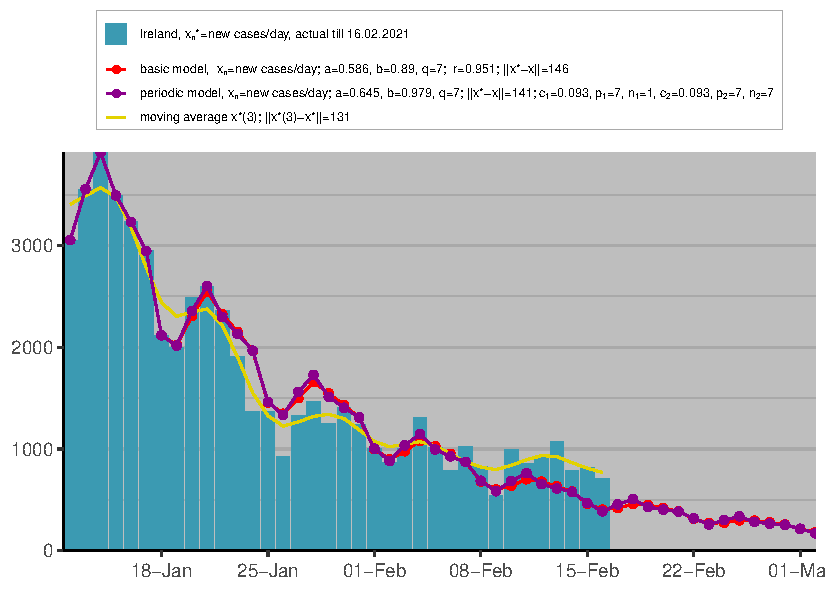
\includegraphics[width=\linewidth]{Ireland-periodic.pdf} \label{fig:ireland-periodic}
\endminipage\hfill
\minipage{0.48\textwidth}
  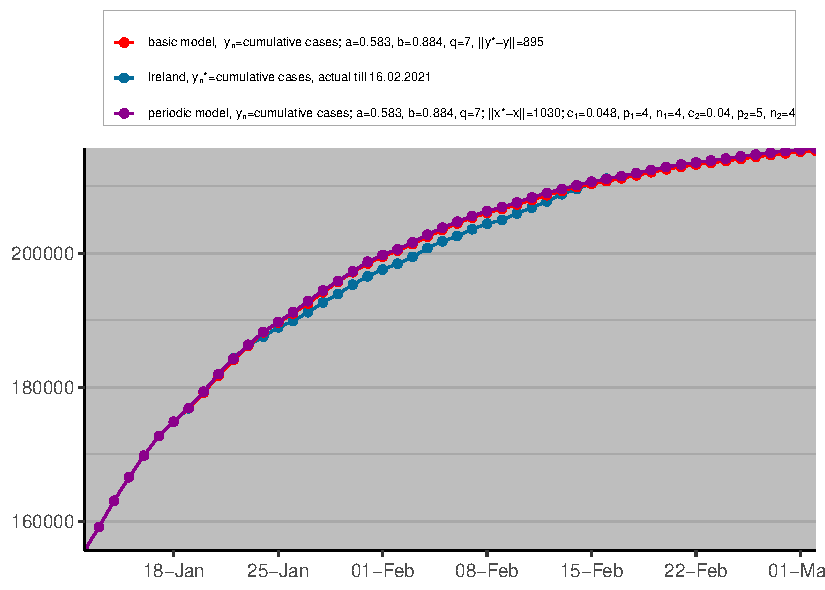
\includegraphics[width=\linewidth]{Ireland-periodicy.pdf} \label{fig:ireland-periodicy}
\endminipage
\caption{Periodic model, Ireland}
\end{figure}

\begin{figure}[H]
\minipage{0.48\textwidth}
  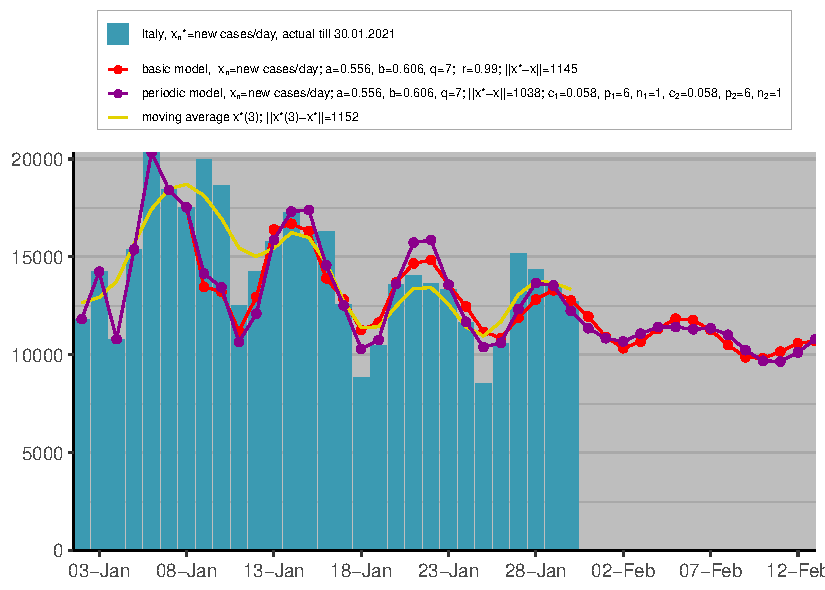
\includegraphics[width=\linewidth]{Italy-periodic.pdf} \label{fig:italy-periodic}
\endminipage\hfill
\minipage{0.48\textwidth}
  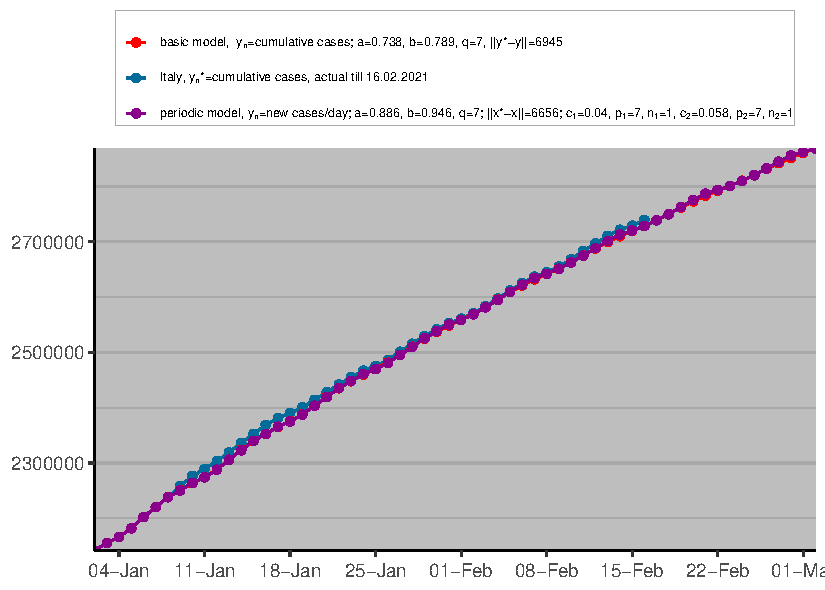
\includegraphics[width=\linewidth]{Italy-periodicy.pdf} \label{fig:italy-periodicy}
\endminipage
\caption{Periodic model, Italy}
\end{figure}

\begin{figure}[H]
\minipage{0.48\textwidth}
  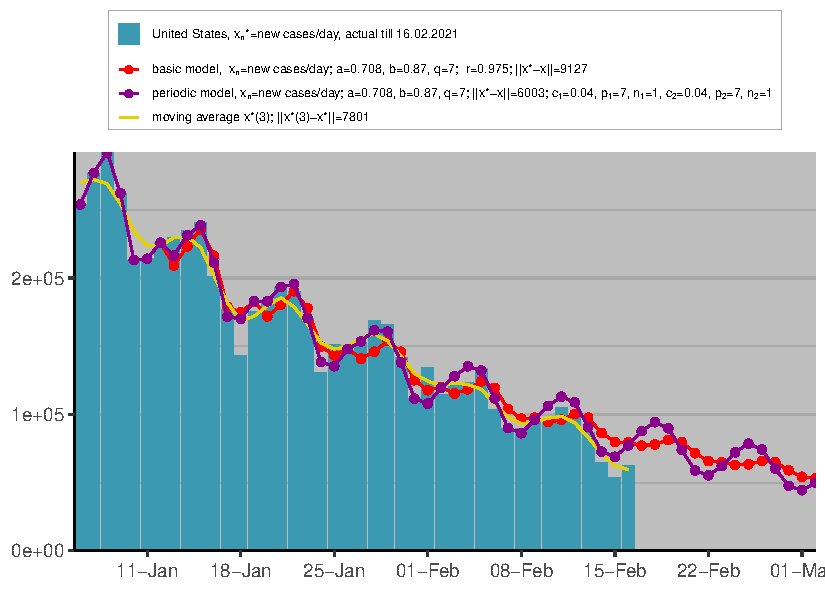
\includegraphics[width=\linewidth]{United States-periodic.pdf} \label{fig:usa-periodic}
\endminipage\hfill
\minipage{0.48\textwidth}
  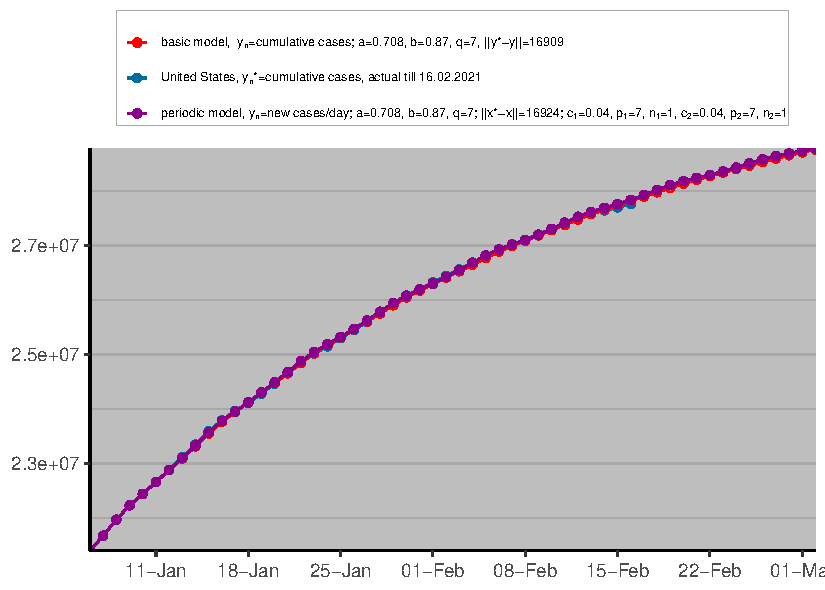
\includegraphics[width=\linewidth]{United States-periodicy.pdf} \label{fig:usa-periodicy}
\endminipage
\caption{Periodic model, United States}
\end{figure}

\subsection{Multi-phase model}

\subsubsection{Definitions and Theory}

\subsubsection{How to select the best model}

\subsubsection{Forecasting}

\subsubsection{Implementation in R}

\subsubsection{Plots}

The multi-phase model without periodicity can be sharp and unrealstic

\begin{figure}[H]
\minipage{0.48\textwidth}
  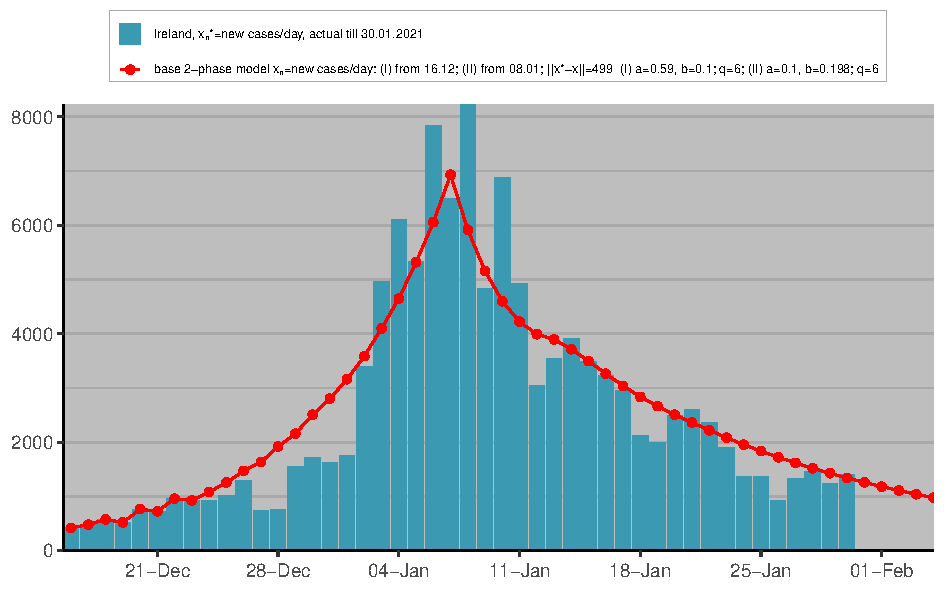
\includegraphics[width=\linewidth]{Ireland-xnmult.pdf} \label{fig:ireland-xnmult}
\endminipage\hfill
\minipage{0.48\textwidth}
  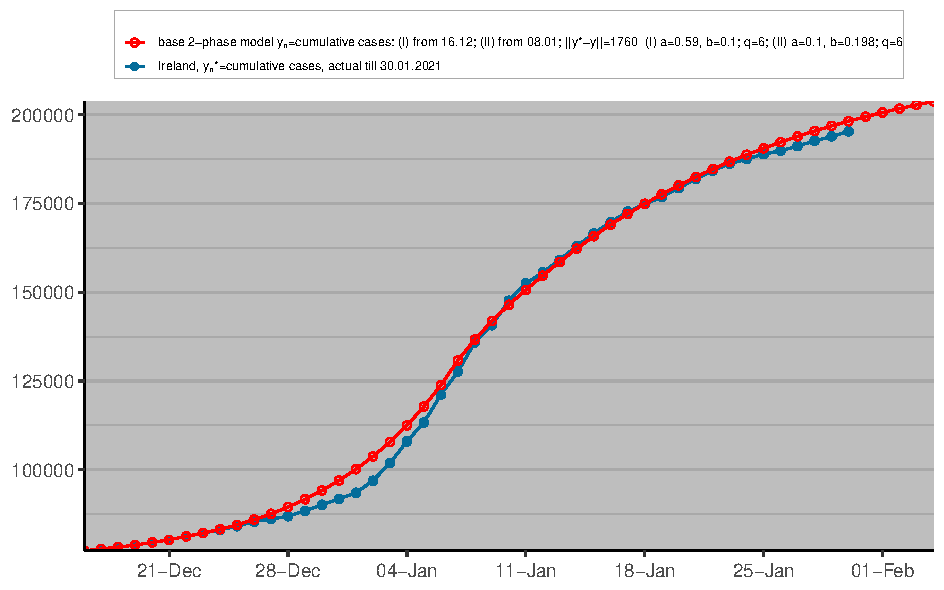
\includegraphics[width=\linewidth]{Ireland-ynmult.pdf} \label{fig:ireland-ynmult}
\endminipage
\caption{Multi-phase model, Ireland}
\end{figure}

\begin{figure}[H]
\minipage{0.48\textwidth}
  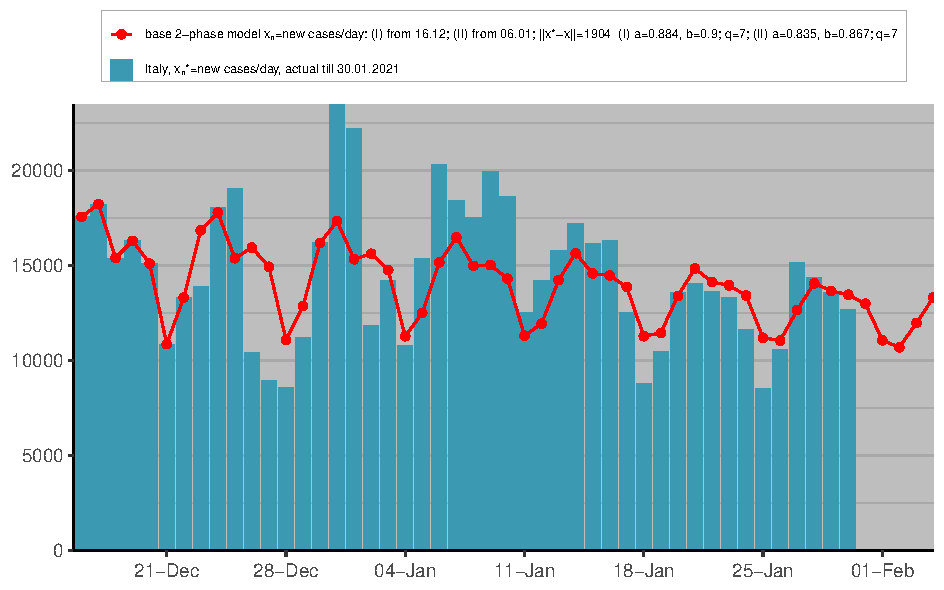
\includegraphics[width=\linewidth]{Italy-xnmult.pdf} \label{fig:italy-xnmult}
\endminipage\hfill
\minipage{0.48\textwidth}
  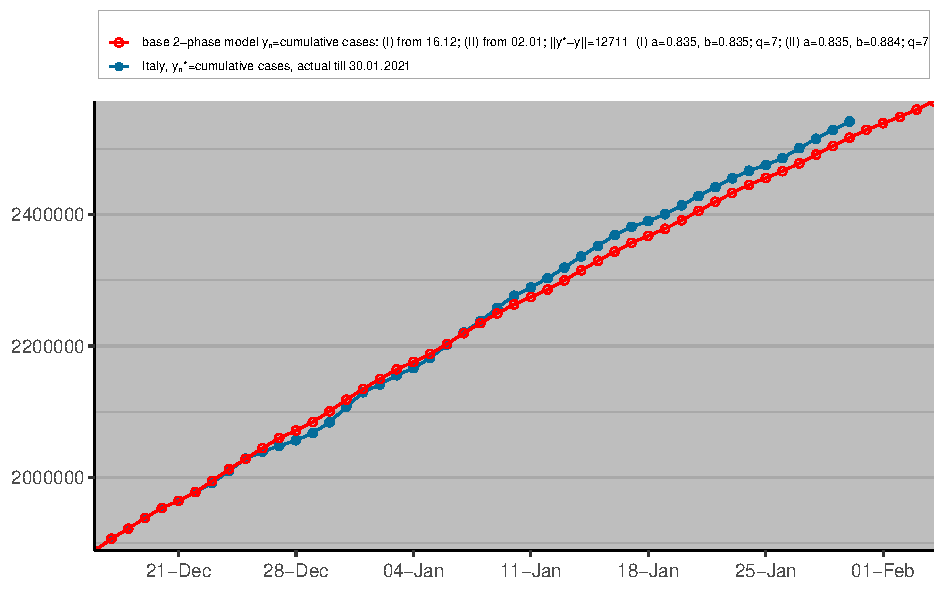
\includegraphics[width=\linewidth]{Italy-ynmult.pdf} \label{fig:italy-ynmult}
\endminipage
\caption{Multi-phase model, Italy}
\end{figure}

\begin{figure}[H]
\minipage{0.48\textwidth}
  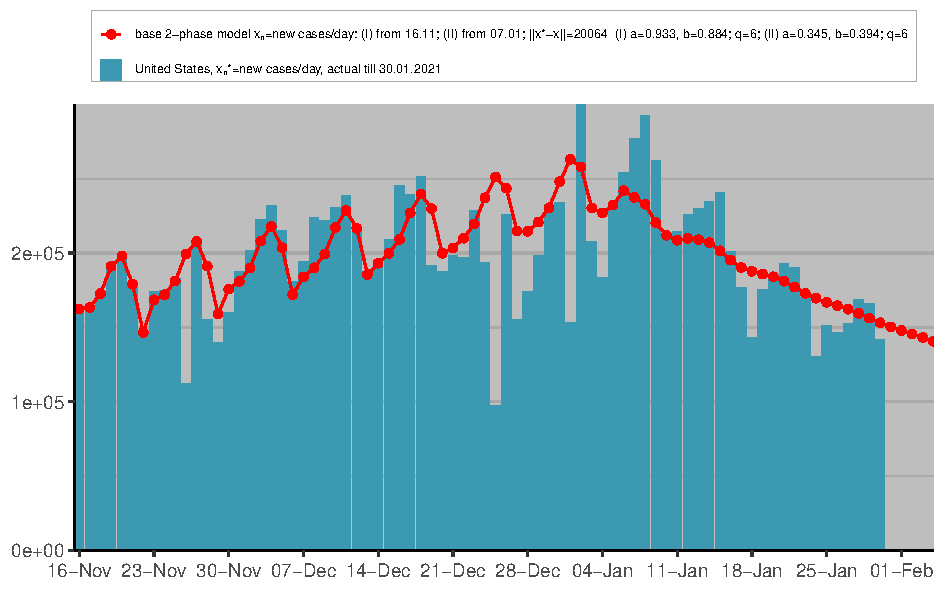
\includegraphics[width=\linewidth]{United States-xnmult.pdf} \label{fig:usa-xnmult}
\endminipage\hfill
\minipage{0.48\textwidth}
  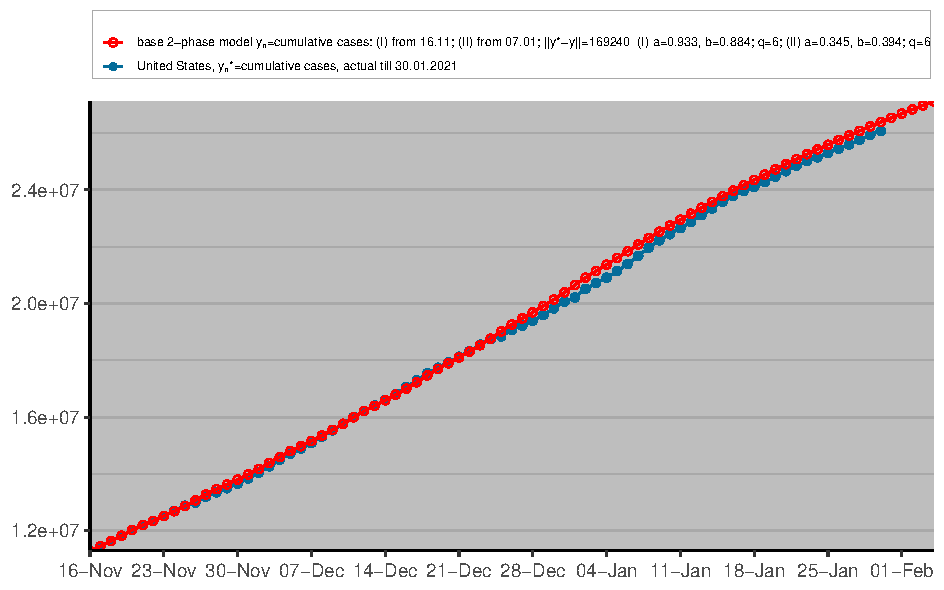
\includegraphics[width=\linewidth]{United States-ynmult.pdf} \label{fig:usa-ynmult}
\endminipage
\caption{Multi-phase model, United States}
\end{figure}


The periodic model often performs much better

\begin{figure}[H]
\minipage{0.48\textwidth}
  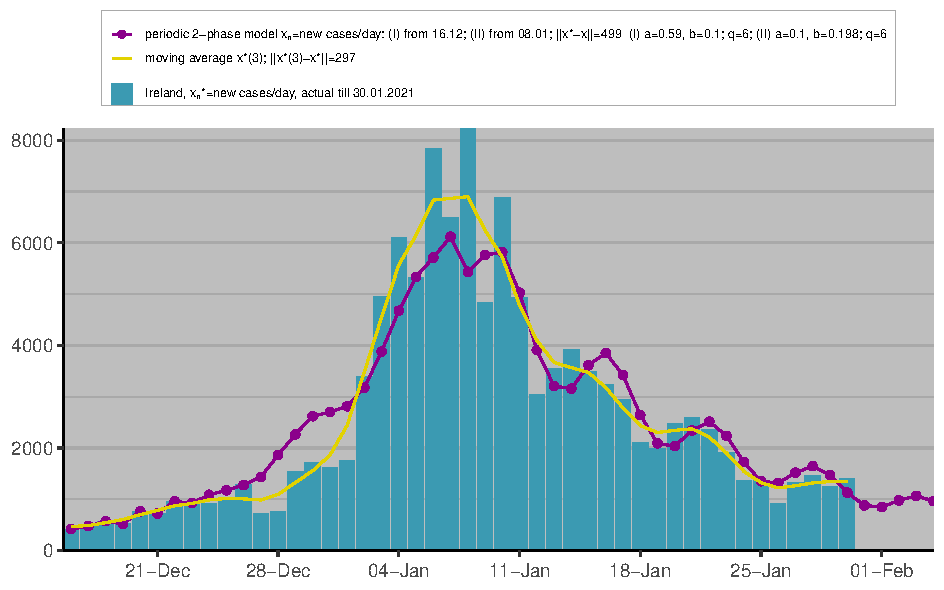
\includegraphics[width=\linewidth]{Ireland-perxnmult.pdf} \label{fig:ireland-perxnmult}
\endminipage\hfill
\minipage{0.48\textwidth}
  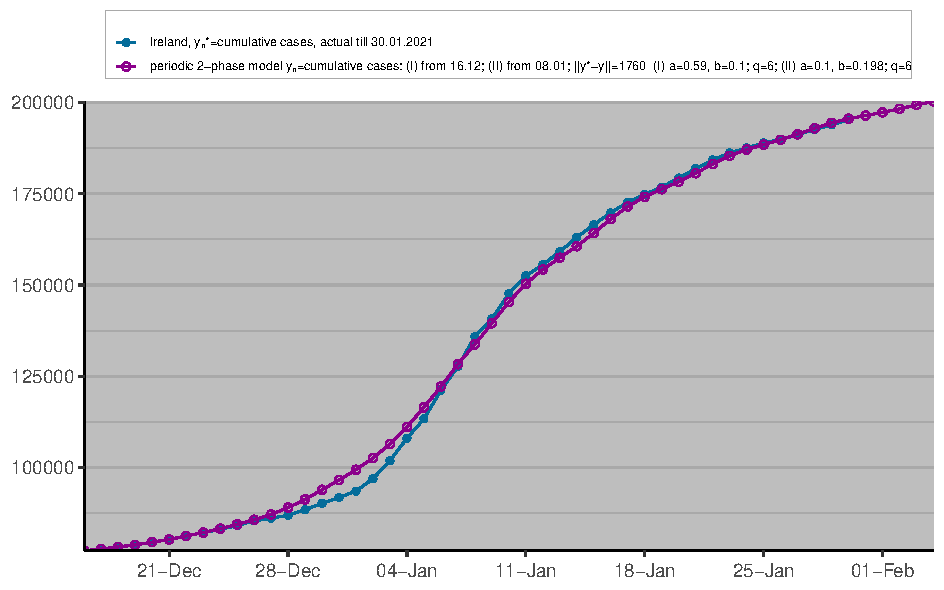
\includegraphics[width=\linewidth]{Ireland-perynmult.pdf} \label{fig:ireland-perynmult}
\endminipage
\caption{Multi-phase periodic model, Ireland}
\end{figure}

\begin{figure}[H]
\minipage{0.48\textwidth}
  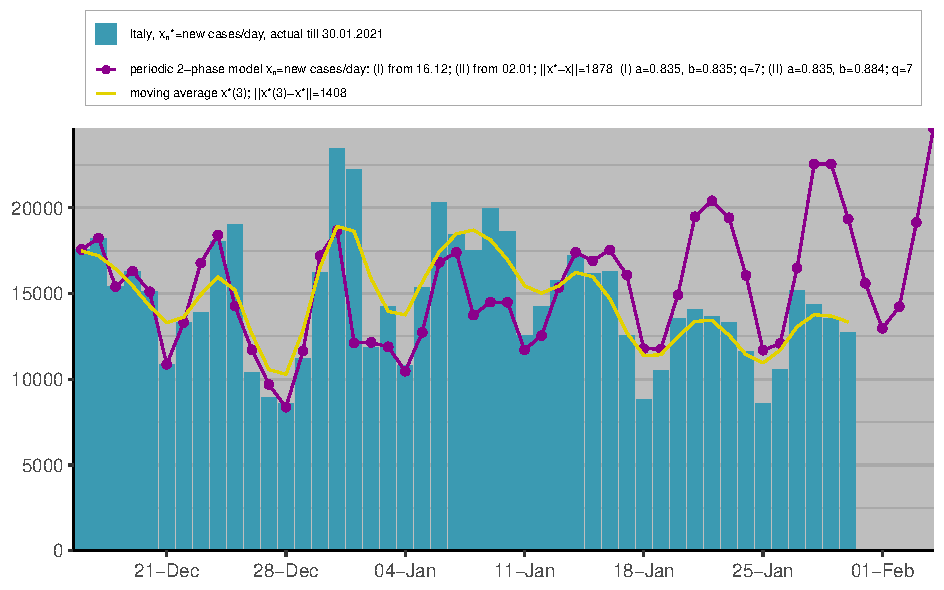
\includegraphics[width=\linewidth]{Italy-perxnmult.pdf} \label{fig:italy-perxnmult}
\endminipage\hfill
\minipage{0.48\textwidth}
  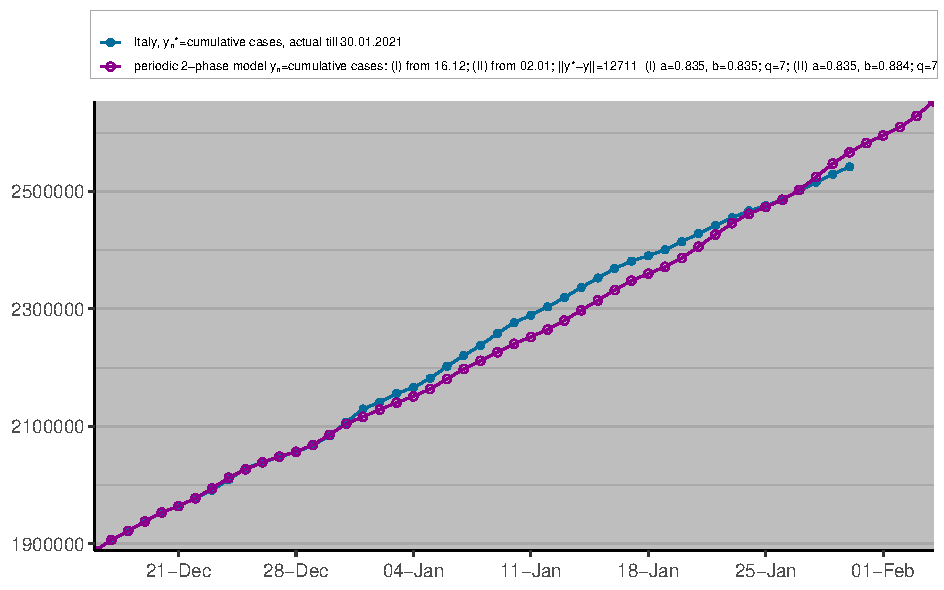
\includegraphics[width=\linewidth]{Italy-perynmult.pdf} \label{fig:italy-perynmult}
\endminipage
\caption{Multi-phase periodic model, Italy}
\end{figure}

\begin{figure}[H]
\minipage{0.48\textwidth}
  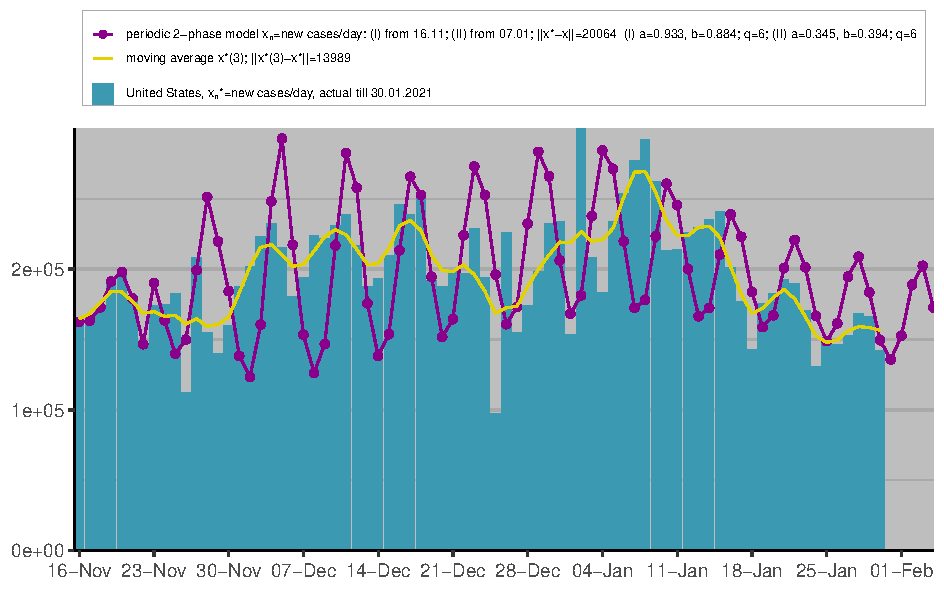
\includegraphics[width=\linewidth]{United States-perxnmult.pdf} \label{fig:usa-perxnmult}
\endminipage\hfill
\minipage{0.48\textwidth}
  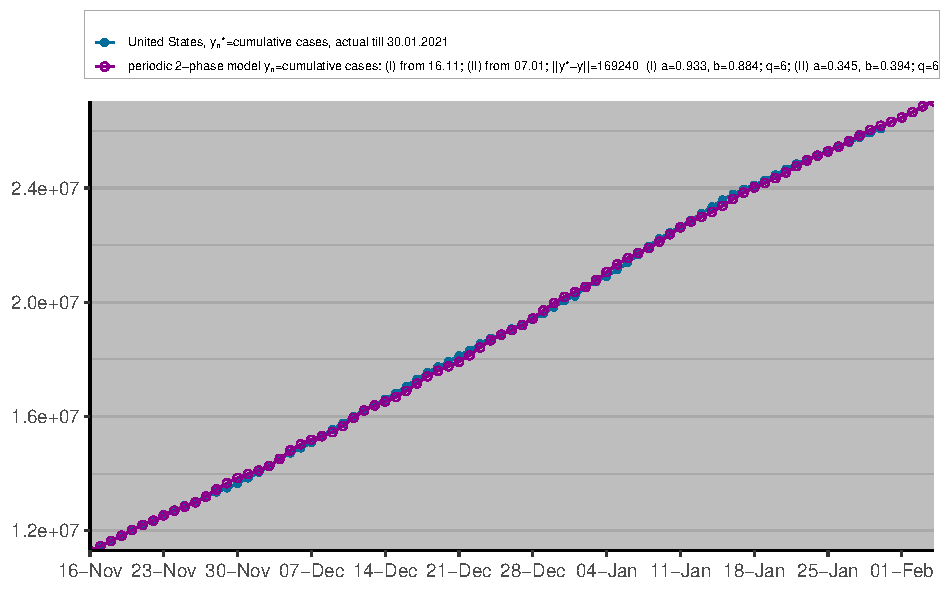
\includegraphics[width=\linewidth]{United States-perynmult.pdf} \label{fig:usa-perynmult}
\endminipage
\caption{Multi-phase periodic model, United States}
\end{figure}
